\documentclass{article}
\usepackage[utf8]{inputenc}
\usepackage{polski}
\usepackage{float}
\usepackage{hyperref}
\usepackage{graphicx}
\usepackage{rotating}
\usepackage{tikz}
\usepackage{amsmath}
\usepackage{subfig}
\usepackage{relsize}
\usepackage{lmodern}
\usepackage{authblk}
\usepackage[a4paper, left=0.9cm, right=0.9cm, top=2.0cm, bottom=2.0cm, headsep=1.2cm]{geometry}

\title{cft-praca1}
\author{m.b.kruk }
\date{March 2019}

\begin{document}

\section{Introduction}
    %The very first observation of fluctuations have just been reported.
    The physics of Bose-Einstein condensation was intensively studied since the appearance of the first papers published in the twenties~\cite{bose1924plancks}~\cite{einstein1924quantentheorie}. Theoretical research investigated not only population of the condensate but also its fluctuations. The problem of the latter turned out to be more troublesome. E. Schrodinger was the first to observe that the standard theory of noninteracting gas in the grand canonical ensemble predicts unphysically large fluctuations~\cite{schrodinger1989statistical}. Later on, it was noted that there is an inconsistency in fluctuations obtained in different statistical ensembles~\cite{ziff1977ideal}. 
    
    The new era of BEC studies begun in 1995, when the rubidium and sodium gases were condensed in laboratories~\cite{davis1995bose}~\cite{anderson1995observation}. Papers concerning canonical~\cite{politzer1996condensate} and microcanonical~\cite{navez1997fourth} ensemble fluctuations in experimentally relevant case of harmonic trap appeared shortly after. 
    These results were followed by studies of interacting gases in the later years ~\cite{bienias2011statisticala}~\cite{bienias2011statistical}~\cite{PhysRevA.93.023636}~\cite{PhysRevLett.97.190402}~\cite{PhysRevLett.82.4376}. Its worth stressing that there are still many open questions in this area. These results are inconclusive, for details see~\cite{kristensen2019observation}.
    
    Over ten years ago, local density fluctuations of quasi-1D Bose gas were measured ~\cite{esteve2006observations}. However, up until now, there was no experimental data concerning fluctuations of the population of the condensate. The recent first measurements of fluctuations ~\cite{kristensen2019observation} revive the interest in the problem of fluctuations of weakly interacting Bose gas.
    
    In this paper, we present detailed studies of statistical fluctuations of the interacting Bose gas confined to a toroidal trap. This makes the system effectively one dimensional.
    % Moreover, we are also investigating the impact of the long-distance dipolar forces on these fluctuations. 
    %In this paper we consider one-dimensional  interacting gas of bosons in a toroidal trap.
     Such form of potential has been succesfully realized in experiment ~\cite{meinert2015probing}.
     
     We analyze two types of interaction between particles: contact and dipolar long range as defined in ~\cite{sinha2007cold}~\cite{PhysRevA.61.041604}. % ~\cite{dipolPotential luis santos, chinskie prace, praca Pawlowski ciemne solitony, praca o ciemnych solitonach z Anglikami, N.Parker wyprowadzil dla dowolnej orientacji}.
    For dipolar interaction both attractive and repulsive character can be achieved by proper orientation of dipoles on the ring. 
    In case of repulsive interactions we study number of atoms in the condensate and its fluctuations as a function of the temperature. For an attractive case i.e in the presence of bright solitons we investigate local density fluctuations and analyze the movement of solitons on the ring.
\section{Model}
    Hamiltonian of the system we consider in this paper reads
    \begin{equation}
    \label{H}
        \hat{H} = \int \mathrm{d}x \; {\hat{\psi}}^{\dag}(x) \frac{\hat{p}^2}{2m} \hat{\psi}(x) + \int \int \mathrm{d}x \mathrm{d}x' \; {\hat{\psi}}^{\dag}(x) {\hat{\psi}}^{\dag}(x') \hat{V}(x-x')\hat{\psi}(x') \hat{\psi}(x)
    \end{equation}
    
    In order to cope with difficult problem of interacting particles we employ the classical fields approximation (for details see~\cite{brewczyk2007classical}) , which we can tune to give us correct macroscopic state functions, provided we choose the optimal cutoff.
    The use of a such approximation corresponds to use Maxwell equations instead of QED in the case of light, therefore cutoff is necessary to avoid situation analogous to UV catastrophe known in the theory of black-body radiation.
    
    The main idea behind classical fields approximation is to replace creation and annihilation operators by complex amplitudes and to neglect modes with value of momentum higher than cutoff momentum $k_{max}$. Atomic field within the classical fields approximation:
    \begin{equation}
        \psi (x) = \sum _{-k_{max}} ^{k_{max}} \alpha  _k \varphi _k (x)=\sum _{-k_{max}} ^{k_{max}}  \frac{1}{\sqrt{L}} \alpha _k e^{ikx}
    \end{equation}
    where $\varphi _k$ are single-particle eigenfunctions of the circular potential and $k=\frac{2 \pi n}{L}, n=0,\pm 1,... , \pm n_{max}$. From now we will use $\epsilon \equiv \frac{2 \pi ^2 \hbar ^2}{m L^2}$, $\hbar/ \epsilon$ and $L$ as units of energy, time and length respectively. Hamiltonian as a function of the complex amplitudes
    \begin{equation}
    \label{Halpha}
        H=\sum_{j=-n_{max}}^{n_{max}}j^2|\alpha _j|^2+\frac{1}{2} \sum_{j_1,j_2,j_3,j_4}C_{j_1,j_2,j_3,j_4} \alpha^*_{j_1}\alpha^*_{j_2}\alpha_{j_3}\alpha_{j_4}
    \end{equation}
    where
    \begin{equation}
        C_{j_1,j_2,j_3,j_4}=\int\displaylimits_0^{1}\int\displaylimits_0^{1}\mathrm{d}x \mathrm{d}x' \; e^{2 \pi i (j_3-j_1)x} \;V(x-x') \; e^{2 \pi i (j_4-j_2)x'}
    \end{equation}
    Plugging hamiltonian \ref{H} into the Heisenberg equation leads to following set of equations of motion for complex amplitudes $\alpha _k$
    \begin{equation}\label{eqs}
        i \frac{\mathrm{d} \alpha_k}{\mathrm{d} t}=k^2 \alpha_k +\sum_{j_1,j_2,j_3}C_{j_1,k,j_2,j_3}\alpha^*_{j_1}\alpha_{j_2}\alpha_{j_3}
    \end{equation}
    We consider contact interparticle potential $V(x-x')=g \delta (x-x')$ and quasi-1D dipole-dipole interaction potential 
    \begin{equation}
    \label{ddi}
        V_{dd}(x-x')=g \; \frac{1}{4l_{\perp}}\Big(-2|\frac{x-x'}{l_{\perp}}|+e^{\frac{1}{2}|\frac{x-x'}{l_{\perp}}|^2}\sqrt{2 \pi}\big(1+|\frac{x-x'}{l_{\perp}}|^2\big)\text{Erfc}\big(|\frac{x-x'}{\sqrt{2}l_{\perp}}|\big)\Big)
    \end{equation}
     with dependency on $l_{\perp}=\sqrt{\frac{\hbar}{m \omega _{\perp}}}$ where $\omega _{\perp}$ is the frequency of harmonic trap responsible for transversal confinement of particles. Note that at the same time length $l_{\perp}$ is directly related to the width of the potential \ref{ddi} ~\cite{deuretzbacher2010ground}, and the potential is normalized to parameter $g$ measuring the strength of the interactions. For $x \gg 0  \quad V_{dd}(x) \sim \frac{1}{x^3}$ as for the standard dipole potential. The full formula for quasi-1D potential contains additional $\delta$-interaction term. However, we want to focus on differences between short and long-range interactions, that is why we consider the situation where this term can be neutralized. 
    One can achieve this by proper tuning of Feshbach resonances leading to the cancellation of $\delta$ terms.
     Due to periodic boundary conditions, the expression for long-range potential \ref{ddi} should be modified 
     \begin{equation}
         V_{per}(x-x')=\sum_{n=-\infty}^{\infty} V(x-x'-n)
     \end{equation}
     \subsection{Cutoff}
    Cutoff parameter $k_{max}$ plays an important role in our calculations. To determine its optimal value we use similar approach to ~\cite{witkowska2009bose}~\cite{witkowska2010monte}. We consider noninteracting gas of $N$
    bosons and calculate probability distribution $P(N_{ex})$  of having $N_{ex}$ excited atoms within canonical ensemble. In Appendix we derive formulas for $P({N_{ex}})$ both exactly (with discrete occupation of energy levels) and in the classical fields approximation.
    \begin{equation*}
        P_{exac}(N_{ex})=\frac{e^{-\beta E_0 N_0}\sum_{k=1}^{\infty} e^{-\beta E_k N_{ex}} \prod_{\substack{j=1\\j \neq k}}^{\infty} \frac{1}{(1-e^{-\beta(E_j-E_k)})^2}\Bigg(N_{ex}+1 + 2\sum_{\substack{l=1\\l \neq k}}^{\infty} \frac{1}{1-e^{-\beta(E_k-E_l)}} \Bigg)}{e^{-\beta E_0 N} \prod _{j=1}^{\infty} \frac{1}{(1-e^{-\beta(E_j-E_0)})^2}+\sum_{k=1}^{\infty}\frac{e^{-\beta E_k N}}{1-e^{-\beta(E_0-E_k)}}\prod_{\substack{j=1\\j \neq k}}^{\infty} \frac{1}{(1-e^{-\beta(E_j-E_k)})^2} \Bigg( N+1 +\frac{1}{1-e^{-\beta (E_k-E_0)}}+2\sum_{\substack{l=1\\l \neq k}}^{\infty} \frac{1}{1-e^{-\beta(E_k-E_l)}} \Bigg)}
    \end{equation*}
     \begin{equation*}
        P_{cl}(N_{ex})=\frac{e^{-\beta E_0 N_0}\sum_{k=1}^n e^{-\beta E_k N_{ex}} \prod_{\substack{j=1\\j \neq k}}^n \frac{1}{(\beta E_k -\beta E_j)^2} \Bigg(N_{ex}+2\sum_{\substack{l=1\\l \neq k}}^n \frac{1}{\beta E_k-\beta E_l}\Bigg)}{e^{-\beta E_0 N} \prod_{j=1}^n \frac{1}{(\beta E_0 -\beta E_j)^2}\\-\sum_{k=1}^n  \frac{e^{-\beta E_k N}}{\beta E_k- \beta E_0} \prod_{\substack{j=1\\j \neq k}}^n \frac{1}{(\beta E_k -\beta E_j)^2}\Bigg(N+2\sum_{\substack{l=1\\l \neq k}}^n \frac{1}{\beta E_k-\beta E_l}+ \frac{1}{\beta E_k -\beta E_0}\Bigg) }
    \end{equation*}
    Optimal cutoff corresponds to the situation, where these two distributions match each other.
    \begin{figure}[H]
        \centering
        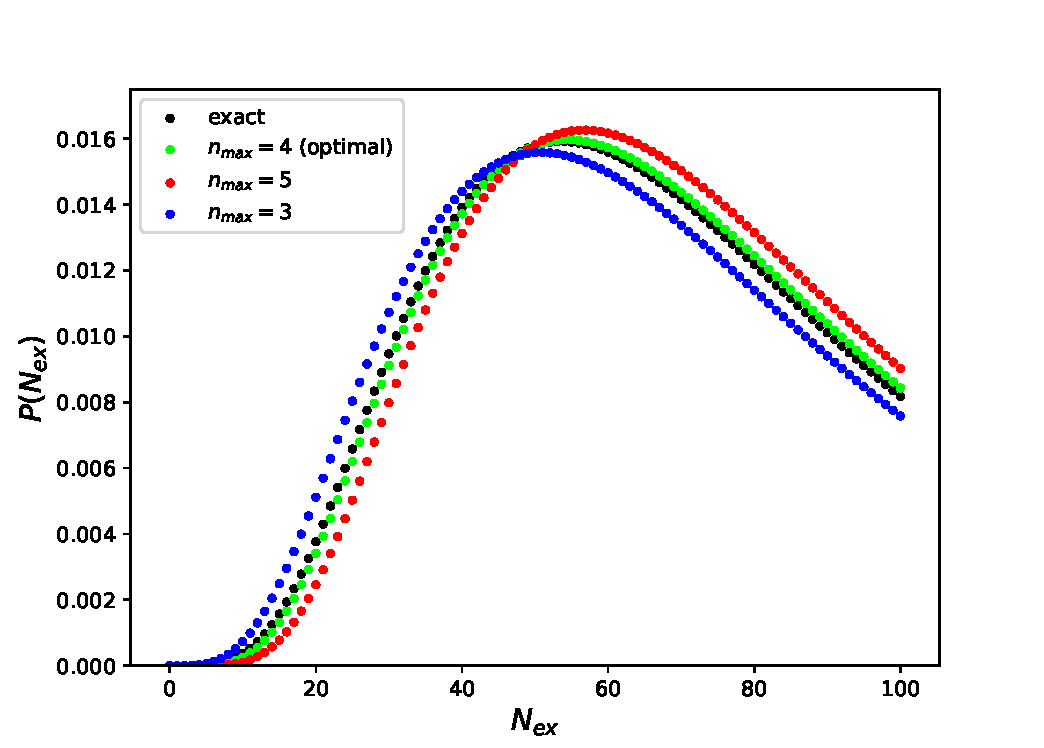
\includegraphics{distcomp.pdf}
    \end{figure}
    Comparing $P_{exac}(N_{ex})$ and $P_{cl}(N_{ex})$ led us to the conclusion that cutoff parameter should be determined from following relation
    \begin{equation}
    \label{eq:cutoff}
    n_{max} = \sqrt{C k_B T}
    \end{equation}
    with $C=0.58$.
 
 
 \section{Method}
     In this paper we will use canonical ensemble for a system described with classical fields approximation. To obtain estimates of statistical properties we sample the ensemble with a Monte Carlo algorithm.
     
     First, to get the states from the thermal equilibrium distribution of the canonical ensemble we decided to use Metropolis alorithm \cite{metropolis1953equation} and implemented it as described in \cite{metropolisImplementation} with code available here \cite{repoLink}. We have confronted these results to those  obtained from the time evolution of equations \ref{eqs}.
    
    The equations of motion look similar to those studied by Fermi, Pasta and Ulam ~\cite{fermi1955studies}. For contact interactions, they are strictly equivalent to equations describing system of nonlinear oscilators with periodic boundary conditios within narrow packet approximation~\cite{berman1984limit}. Furthermore, for contact interactions they can be seen as set of equations describing evolution of Fourier amplitudes of function $\psi(x)$ satisfying periodic Nonlinear Schrodinger equation (NLS). NLS is known to be completely integrable ~\cite{berman1984limit}. This fact may question the ergodicity of our system. Three constants of motion have clear interpretation of energy, momentum and the number of particles. That is why we can think of time-averaged quantities as quantities obtained in a microcanonical ensemble further constrained by the constant momentum and the remaining constants of motion.

\section{Repulsive gas}
    We use two different approaches to obtain average number of atoms in condensate and its fluctuations for a given temperature. The first one uses Metropolis algorithm ~\cite{metropolis1953equation} to generate canonical ensemble probability distribution. The second one consists of calculating time averages from time dependencies obtained by solving equations \ref{eqs}.
    
     Initial conditions for the evolution were chosen from the set of states generated by the Monte Carlo algorithm in a way such that the energy of the state was the closest to equilibrium value and the momentum was closest to zero. Two states randomly selected in this way may differ in values of other constants of motion, which in turn may lead to very different values of time-averaged quantites. However, we've observed that for sufficiently strong interactions time averaged fluctuations and populations don't depend on choice of initial condintions provided the energy and momentum is the the same.
     
    Microcanonical ensemble, as well as our equations, do not involve temperature.
    Thus, the temperature in case of time evolution should not be seen as a physical parameter, but rather as an indicator telling us that the evolution was performed for the  occupation of modes and energy characteristic for a system in equilibrium at the temperature T.
    
    The interaction strength used for simulations was $g=0.5$. In order to check whether this value corresponds to the regime of weakly interacting gas, we've calculated depletion of the condensate in $T=0$ within the standard Bogoliubov approximation. The depletion turned out to be around 14 percent.

\section{Attractive gas}
   Now we turn to the attractive gas. In low-temperature regime we expect quasicondensate and bright solitons in density profile of the gas. Quasicondensation refers to the situation where there is no single dominant eigenvalue of one-particle density matrix. In other words, there is more than one mode with with macroscopic population. We observe such phenomenon in results of Monte Carlo simulations, where even for very weak interactions condensate population is around 50 percent for the lowest temperature. Due to the dimensionality of the system, quasicondensate occurs also for repulsive gas but is not as drastic as in the case of attractive interactions.

\subsection{Hartree-Fock, variational method}
    Unlike for the repulsive interaction the ground state is not uniform. Thus, the choice of the cutoff should be modified.
    To find the ground state for attractive gas of $N$ particles we emply two methods -- analytical approximation and numerical algorithm. One can expect that the wave function of the ground state will take a localized shape due to the attractive interaction. Basing on this assumption we take the wave function of the following form
    $$ \psi(x_1,...,x_N) =\prod _{j=1}^N \varphi(x_j), \qquad \varphi(x)=\frac{1}{\sqrt{\sqrt{\pi}\lambda}} \text{e}^{-\frac{1}{2}(\frac{x}{\lambda})^2} $$
    with a free parameter $\lambda$ describing the width of the wave function. We then minimize the energy in this state with respect to $\lambda$. For contact interaction the interaction energy can be computed analytically and is equal
    $$ V_{\delta} = \frac{g N(N-1)}{\sqrt{2 \pi} \lambda} $$
    The total energy reaches minimum for $\lambda =-\frac{1}{ (2 \pi) ^{3/2} g (N-1)} $ and is equal
    $$ E_{\delta} = -\pi g^2 (N-1)^2 N $$
    However, it is not possible to solve analytically the dipole-dipole interaction and thus the energy was computed numerically and the minimimum was found numerically.
    %it Newton's algorithm for $\frac{dE}{d\lambda}$ was used with numerically estimated derivatives.
    Our goal was to modify cutoff in such a way that Monte Carlo simulations at very low temperature reproduce energy and width of the optimal state. This approach is similar to \cite{bienias2011statisticala} and can be expressed in formula
    \begin{equation}
        n_{max}=\sqrt{C k_B T}+n(g)
    \end{equation}
    where $n(g)$ is the number of mode pairs we have to add to reproduce the optimal state. We emphasize that extension of above formula to high temperatures is not obvious.
\subsection{Random walk}
    It is clear that many-body Hamiltonian we consider commutes with the rotation generator. For this reason, the multi-particle wave function of the ground state of the system should not change under rotations. However, when measuring positions of individual particles, one should rather expect localized gaussian-like shape with well-defined position of maximum. Of course, no point on the circle is distuinguished so in the series of measurements, each one should lead to a different position of the soliton. The phenomenon of spontaneous symmetry breaking via measurement was understood over twenty years ago in the case of interference of two condensates ~\cite{javanainen1996quantum}~\cite{andrews1997observation} and more recently, for excited state of 1D repulsive gas ~\cite{syrwid2015lieb}.
    
    In this paper, we take the Metropolis' algorithm and treat each consecutive sample as an element of a discrete time sequence, and show that for the attractive gas the peak of the wave profile exibits Brownian motion properties such as mean distance after $n$ time steps behives like $\sqrt{n}$ and each consecutive pair of changes in positions is not cerrelated. So its really Markovian random walk. However the whole ensemble restores the rotational symmetry because samples don't distuinguish any point on circle.  
    It is interesting to note that within classical fields approximation individual realization of the field are breaking symm and thus corresponds to single measurements.
    
    Then we've provided the equations \ref{eqs} with initial conditions generated by MC algorithm for parameters guarrenteeing presence of bright solitons. The shape of the soliton was preserved during time evolution. We've analyzed the positions of peak obtained in equal time steps. It turned out that the distribution of step length is gaussian, but due to correlation between length of two consecutive steps (peak tend to travel in one direction for quite a long time) we didn't observe characteristic $\sqrt{t}$ behavior of mean distance. 
\subsection{Local density fluctuations}
    For attractive interactions, we study fluctuations of local denisty. For every sample generated by Monte Carlo simulation we consider its density profile.
    
    Every density profile corresponds to a different position of the soliton. That is why using bins with positions fixed relatively to the ring wouldn't lead us to reveal any structure in the distribution of density fluctuations across bins. We use other approach in which we start with determining the maximum of the density profile. Then we divide the ring into bins with respect to the position of the peak. Finally, we collect data from all samples generated with MC algorithm.

\section{Summary}
\bibliographystyle{unsrt}
\bibliography{bibliography.bib}
\end{document}

Feshbach w pierwszych pracach o solitonach. Napisac o hamiltonianie i niezm wzgl obrotow. Gaussian zlokalizowany Javanajnen twa stany Foka interferencujnego (cytowanie w pracy o solitonach w 2017). Pojednycze zespoly alf jako pomiar. JEsli jest struktura stanu kwantowego, to moze byc w pojedynczym pomiarze, nie w calym stanie. Caly stan -> caly zespol. Wazne prace Ketterle i Javainen
